
\section{Shallow-Ice Test Cases}
\label{sc:sia-tests}

These tests are primarily useful for testing the shallow-ice approximation (SIA) dynamical core, Glide (see Chapter~\ref{ch:glide}).
The Glissade dycore also has a shallow-ice option (see Section~\ref{sc:glissade-sia}).

% =====================================
\subsection{Halfar dome}
% =====================================

\label{sec:halfar_description}
The Halfar test case describes the time evolution of a parabolic dome of ice, as described by \citet{Halfar1983}.
For a flat-bedded SIA problem, this case has an analytic solution for the time varying ice thickness. We start with the
general SIA ice evolution equation,  

\begin{equation}
    \label{halfar}
    \frac{\partial H}{\partial t} = \nabla \cdot (\Gamma H^{n+2} |\nabla H|^{n-1} \nabla H),
\end{equation}
%
where $n$ is the exponent in the Glen flow law, commonly taken as 3, and $\Gamma$ is a positive constant:

\begin{equation}
    \Gamma = \frac{2}{n+2} A (\rho g)^n.
\end{equation}
%
For $n=3$, the time-dependent solution is

\begin{equation}
    H(t,r) = H_0 \left(\frac{t_0}{t}\right)^\frac{1}{9}  \left[ 1 - \left(  \left( \frac{t_0}{t} \right) ^ \frac{1}{18} \frac{r}{R_0} \right)^\frac{4}{3} \right] ^ \frac{3}{7},
\end{equation}
%
where

\begin{equation}
    t_0 = \frac{1}{18\Gamma} \left( \frac{7}{4} \right)^3 \frac{R_0^4}{H_0^7},
\end{equation}
%
and $H_0, R_0$ are the central height of the dome and its radius at time $t=t_0$.
For more details, see \citet{Halfar1983}, \citet{Bueler2005}, and this \href{http://www.projects.science.uu.nl/iceclimate/karthaus/2009/more/lecturenotes/EdBueler.pdf}{link}\footnote{http://www.projects.science.uu.nl/iceclimate/karthaus/2009/more/lecturenotes/EdBueler.pdf}.

\subsubsection{Provided files}
\label{subsec:halfar_files}

Our implementation of the Halfar dome test has an initial radius of $R_0=21.2$ km and an initial thickness of $H=707.1$ m.
These values can be changed by editing \texttt{halfarDome.py}.

\begin{itemize}
	\item README \\
		Information about the test case, including technical details about running it.
	\item halfar.config \\
	        This is the config file defining CISM options. It is set up to run Glide. \\
  \item halfarHO.config \\
              This alternative config file is set up to run Glissade
              using the Blatter-Pattyn approximation of Stokes flow. By manually setting
              \texttt{which\_ho\_approx} under \texttt{[ho\_options]}, users can choose other approximations 
              (see Section~\ref{ug.sec.config}).
	\item halfar.py \\
		This python script generates the dome initial condition and runs CISM.
	\item halfar\_results.py \\
		This script compares model results to the analytic solution.
	\item halfarDome.py \\
		This python module defines the analytic solution. \\
    		 It is not meant to be run manually, but is used by the other scripts.
\end{itemize}

\subsubsection{Running the test}
One script sets up the initial condition and runs the model:

\texttt{./halfar.py}

Note that to run the test with the \texttt{halfarHO.config} settings, you can use
the \texttt{-c} commandline option for specifying a configuration file:

\texttt{./halfar.py -c halfarHO.config}

Another script analyzes and plots the results:

\texttt{./halfar\_results.py}

\subsubsection{Results}
\label{subsecc:halfar_results}
With the default .config settings, this simulation should only take a few seconds and is a good first test for a working Glide dycore.
With Glissade, the Blatter-Pattyn option takes a few minutes, but the SIA and L1L2 settings are much faster.
As the dome of ice evolves, its margin advances and its thickness decreases (there is no surface mass balance to add new mass).  
The script \texttt{halfar\_results.py} will plot the modeled and analytic thickness at a specified time (Figure \ref{fig:halfarresults}), 
and also report error statistics.  Invoke \texttt{halfar\_results.py --help} for details on its use.

\begin{figure}[H]
	\centering
	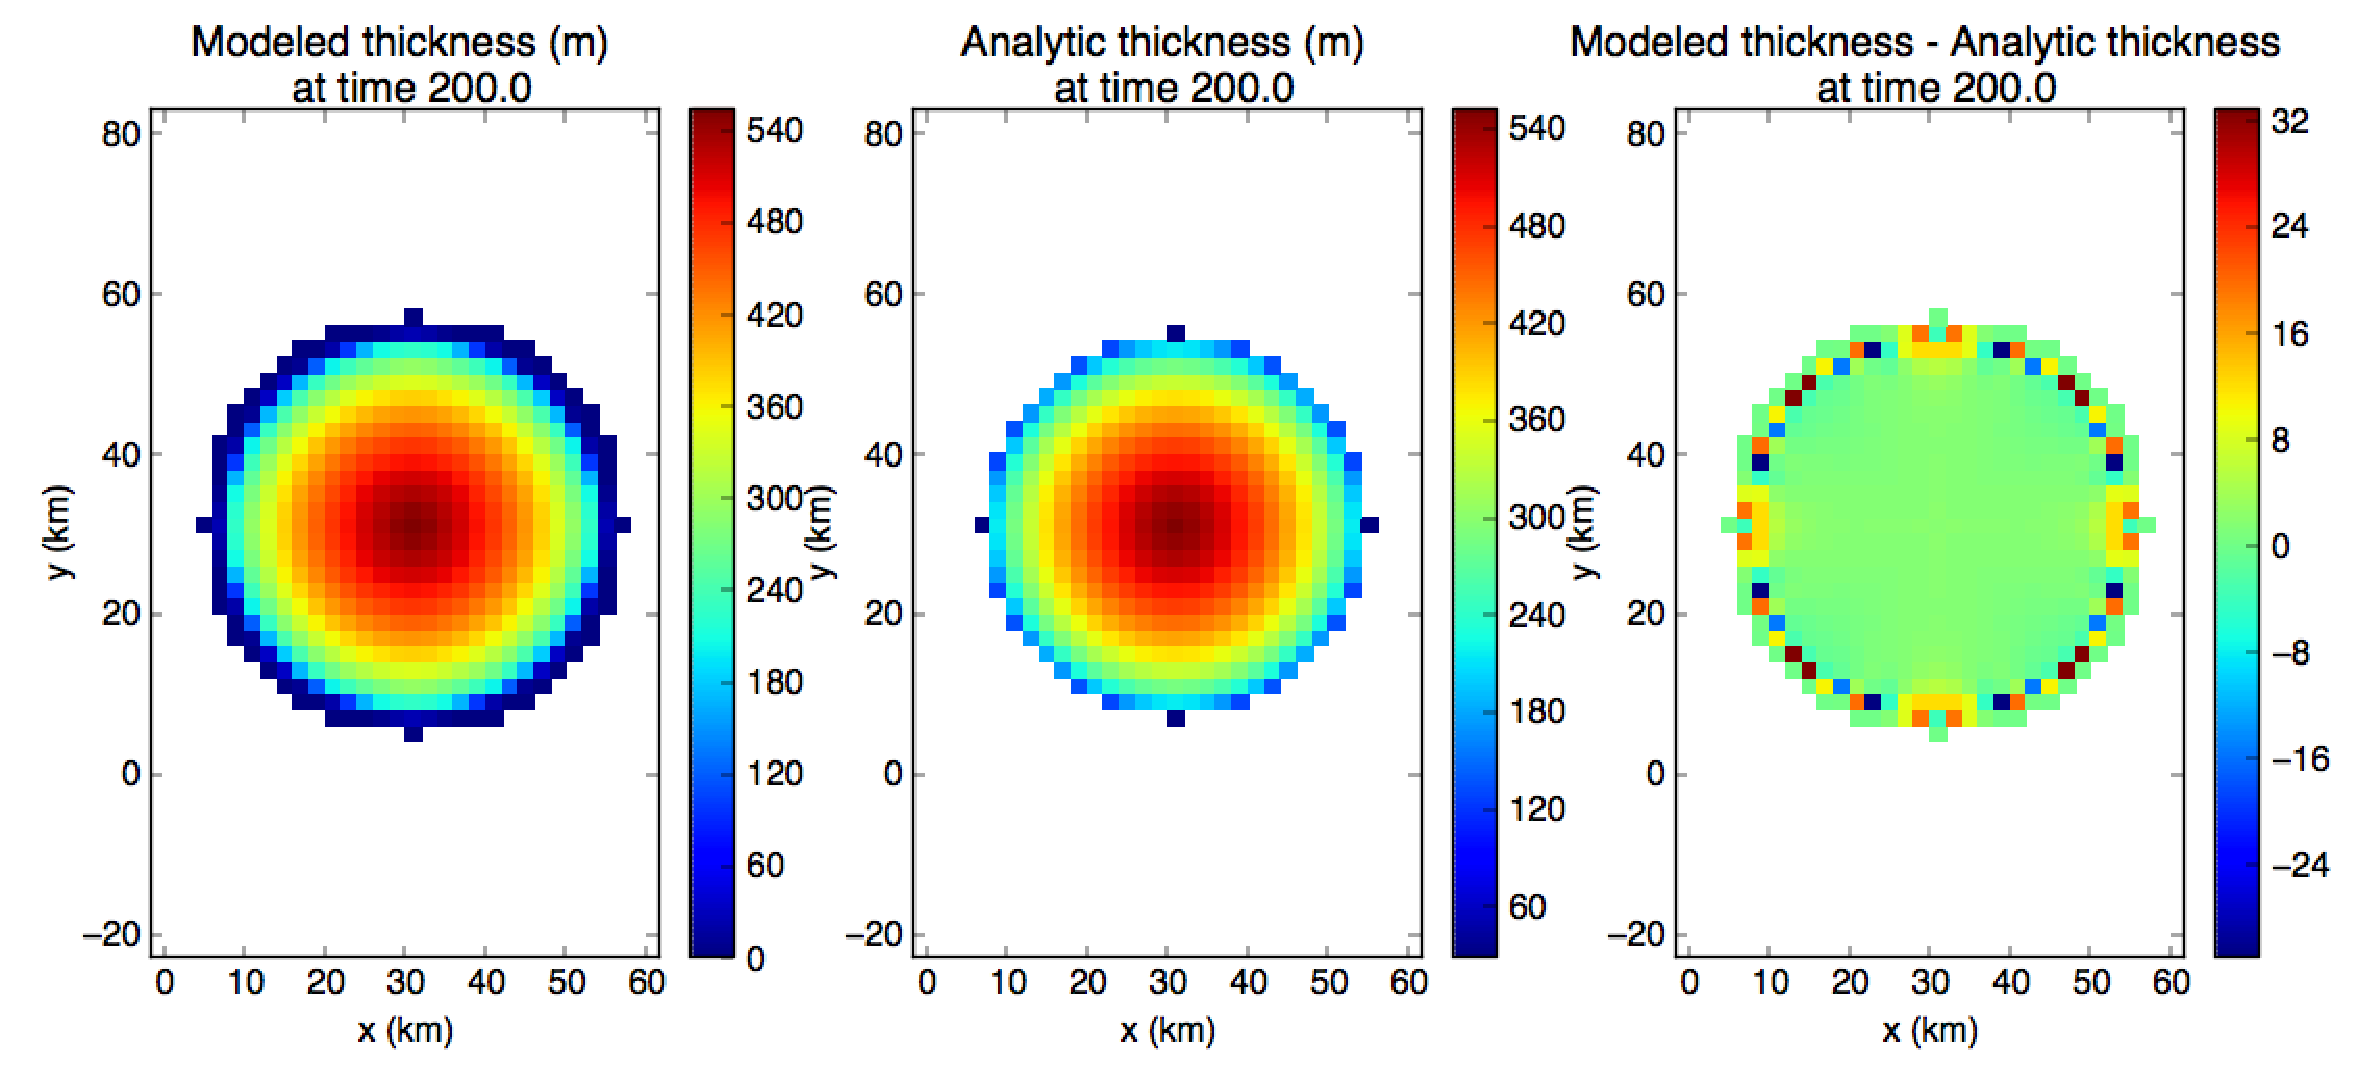
\includegraphics[width=16.4cm]{\dir/halfar_results.eps}
	\caption{Halfar test case results (using Glide) after 200 years of dome evolution. This figure is generated by \texttt{halfar\_results.py}.}
	\label{fig:halfarresults}
\end{figure}


\FloatBarrier


% =====================================
\subsection{EISMINT-1}
% =====================================
\label{sec:eismint_description}
This test case is from phase 1 of the European Ice Sheet Modelling INiTiative intercomparison experiments.  These experiments are described in more detail
\href{http://homepages.vub.ac.be/~phuybrec/eismint.html}{here}\footnote{http://homepages.vub.ac.be/\textasciitilde{}phuybrec/eismint.html} and in \citet{Huybrechts1996}.

\subsubsection{Provided files}
\label{subsec:eismint_files}

\begin{itemize}
	\item README \\
	Information about the test case, including technical details about running it.
	\item *.config \\
  	There are .config files for each of the six experiments in EISMINT 1: three fixed margin experiments (fm) and three moving margin experiments (mm).
\end{itemize}

\subsubsection{Running the test}
There is no script for running these experiments. They are simply run manually, e.g. using: 

\texttt{./cism\_driver e1-fm.1.config}

\subsubsection{Results}
\label{subsecc:eismint_results}
These experiments are meant to be run to steady-state, and the supplied .config files are set up to run for long enough to do this.
These simulations take more than a few minutes to complete.
As the ice sheet evolves, its shape eventually equilibrates with the imposed surface mass balance.  
Currently there is no script for analyzing the model results.  
However, users can visually compare their results to those in \citet{Huybrechts1996}.


% =====================================
\subsection{EISMINT-2}
% =====================================
\label{sec:eismint2_description}
This test case is from phase 2 of the European Ice Sheet Modelling INiTiative intercomparison experiments.  These experiments are described in more detail
\href{http://homepages.vub.ac.be/~phuybrec/eismint.html}{here}\footnote{http://homepages.vub.ac.be/\textasciitilde{}phuybrec/eismint.html} and in \citet{Payne2000}.

\subsubsection{Provided files}
\label{subsec:eismint2_files}

\begin{itemize}
	\item README \\
	Information about the test case, including technical details about running it.
  	\item *.config \\
  	There are 11 .config files: one for each of the experiments described in \citet{Payne2000}.
  	\item mound.nc, trough.nc \\
    	These are input netCDF files used by the EISMINT-2 experiments.
\end{itemize}

\subsubsection{Running the test}
There is no script for running these experiments. They are run manually, e.g. using: 

\texttt{./cism\_driver e2.a.config}


\subsubsection{Results}
\label{subsecc:eismint2_results}
These experiments are meant to be run to steady-state, and the supplied .config files are set up to run for long enough to do this.  
Some experiments use the final state of a previous experiment 
as the initial condition (e.g., most experiments following experiment A use the final state from A as an initial condition).  
See the experimental descriptions in \citet{Payne2000} for details.
These simulations take more than a few minutes to complete.
As the ice sheet evolves, its shape equilibrates with the imposed surface mass balance.  
There is no script for analyzing model results, but users can visually compare their results to those in \citet{Payne2000},
and also compare model diagnostics (e.g., ice area, volume, and maximum thickness) to Table 4 of that paper.


% =====================================
\subsection{Glint example}
% =====================================
\label{sec:glint_example}

Section~\ref{ug.use_glint} explains how to set up and run the Glint example test case.
We summarize that information here.

\subsubsection{Provided files}
\label{subsec:glint_files}

\begin{itemize}
	\item README.glint\_example \\
         Information about the test case, including technical details about downloading the required data files
         and running the case.
  	\item greenland\_20km.config.pdd and glint\_example.config.pdd \\
  	 These config files are used to run Glide with the surface mass balance computed by Glint's positive-degree-day scheme.
  	\item greenland\_20km.config.pdd and glint\_example.config.pdd \\
  	 These config files are used to run Glide with the surface mass balance passed directly to Glint.
         (In real applications the SMB would be provided by a climate model, but here it is crudely approximated from
         temperature and precip data.)
  	\item  ncep-doe\_6h\_climate.64x32.nc, orog.igcmgrid.64x32.nc, gland20.input.nc \\
    	 These are data files that must be downloaded and placed in the \texttt{glint\_example} test directory by the user.
         Users may also supply their own input data.
\end{itemize}

\subsubsection{Running the test}
There is no script for running these experiments. They are run manually, e.g. using: 

\texttt{./cism\_driver greenland\_20km.config.pdd glint\_example.config.pdd}

The two config files specify the ice sheet and climate configurations, respectively. 

\subsubsection{Results}

The config files are set up to run Glide on a coarse Greenland grid for 10 model years,
so that the default experiments complete quickly.  The results are written to netCDF files.
This test illustrates the application of CISM to a whole ice sheet but is not expected
to be scientifically accurate.

